% quark_scan_methodology_note.tex
% Why the M_KK envelope plot answered the wrong question, and what the right
% question (and answer) looks like. Aimed at a reader who is not an RS-flavor
% specialist; jargon is defined as it appears.
\documentclass[11pt]{article}

\usepackage[margin=1in]{geometry}
\usepackage{parskip}
\usepackage{amsmath,amssymb}
\usepackage{booktabs}
\usepackage{array}
\usepackage{xcolor}
\usepackage{hyperref}
\usepackage{enumitem}
\usepackage{graphicx}
\usepackage{caption}
\usepackage[font=small,labelfont=bf]{caption}

\hypersetup{colorlinks=true,linkcolor=blue,citecolor=blue,urlcolor=blue}

\graphicspath{{../results/figures/quark/}}

\newcommand{\Mkk}{M_{\mathrm{KK}}}
\newcommand{\LamIR}{\Lambda_{\mathrm{IR}}}
\newcommand{\Mpl}{M_{\mathrm{Pl}}}
\newcommand{\gs}{g_s^{\star}}
\newcommand{\gsfour}{g_s^{(4)}}
\newcommand{\gsfive}{g_s^{(5)}}
\newcommand{\fIR}{f_{\mathrm{IR}}}
\newcommand{\Yu}{Y_u}
\newcommand{\Yd}{Y_d}
\newcommand{\msbar}{\overline{\mathrm{MS}}}
\newcommand{\eK}{\varepsilon_K}
\newcommand{\dmK}{\Delta m_K}
\newcommand{\dmBd}{\Delta m_{B_d}}
\newcommand{\dmBs}{\Delta m_{B_s}}
\newcommand{\dmD}{\Delta m_{D^0}}
\newcommand{\KKgluon}{\mathrm{KK\text{-}gluon}}

\title{Quark Scan: Fitting vs.\ Sampling, and Why\\[2pt]
       the Envelope $\Mkk$ Bound Was So Low}
\author{}
\date{\today}

\begin{document}
\maketitle

\begin{center}
\fcolorbox{red}{yellow!20}{\parbox{0.95\linewidth}{\small
\textbf{LEGACY / SUPERSEDED (May 2026 $\Delta F=2$-only note).}
This note covers only the $\Delta F=2$ flavor sector and predates the June 2026
audit. Its headline flavor-only floors ($47.26$, $127.13$, $44.50$~TeV) and the
CFW factor-$2.2$ reconciliation narrative are \emph{not} the current
project floors and should not be read as such. It also states that the repo
``does not compute oblique parameters, $Zb\bar b$ corrections, or global EWPO''
--- that is no longer true (see \texttt{quarkConstraints/oblique\_stu.py},
\texttt{rs\_ew\_couplings.py}, and the EW001/T010/T011 catalog constraints).
The corrected, authoritative picture: a \emph{typical} minimal floor
$\sim 30$~TeV from $\varepsilon_K$, an \emph{existence} floor $\sim 18$--$20$~TeV
from irreducible oblique $S,T,U$, and $Zb\bar b \sim 5$~TeV after the B1 fix; the
audit reproduces Bauer 0912.1625, Gedalia 0906.1879, and Blanke 0809.1073. See
\texttt{docs/FLOOR\_SUMMARY.md} and
\texttt{reports/collaborator\_2026-06/CONTENT.md}.}}
\end{center}

%% =====================================================================
\section{What the headline outcome is}
\label{sec:summary}

In response to the collaborator's critique, we did two specific things:

\begin{enumerate}[leftmargin=2em,itemsep=2pt]
  \item \textbf{Promoted the quark mass targets to PDG-faithful $\msbar$ values.}
        Previously the scan was matching to ad-hoc numbers nominally evaluated
        at the KK scale ($\sim 3$~TeV); the strange quark target alone was off
        by $\sim 50\%$. We replaced these with the PDG~2024 $\msbar$ masses
        and ran them down to a common reference scale of $\mu = m_t = 163.5$~GeV
        using four-loop QCD mass running with the standard $n_f = 6 \to 5 \to 4$
        threshold matching at the heavy-quark thresholds.
  \item \textbf{Re-ran the dense scan} (100\,k points, $r \in [0.05,1.0]$,
        $\Mkk \in [1,20]$~TeV) under the corrected targets and a tightened
        $2\sigma$ PDG tolerance on both quark masses and the four CKM observables
        $|V_{us}|,\,|V_{cb}|,\,|V_{ub}|,\,J$.
\end{enumerate}

\noindent The publication-style $\Mkk$ exclusion plot from this re-run is
\emph{visually almost identical} to the previous version. The lowest allowed
$\Mkk$ stayed at $\sim 1.2$~TeV in both the old and the corrected scans.
The collaborator was right that the targets had been wrong, and we fixed
them, and the headline $\Mkk$ number did not move.

The rest of this note explains why that is correct, and what we should be
plotting instead.

\medskip
\noindent\textbf{Reading guide.}
\S\ref{sec:np}--\S\ref{sec:gauge-coupling} introduce the physics needed to
read the figures: what ``new physics'' means, what the FCNC ``ratio'' is,
and the gauge-coupling convention that sets the absolute $\Mkk$ scale.
\S\ref{sec:envelope-existence}--\S\ref{sec:envelope-yukawa} explain why
the envelope plot has been answering an existence rather than a typicality
question, and what the optimiser's Yukawas actually look like.
\S\ref{sec:rs-anarchy}--\S\ref{sec:how-anarchic-passes} present the
alternative ``RS-anarchy'' analysis, including where the priors come
from and how a random draw can satisfy PDG masses without any fitting.
\S\ref{sec:result}--\S\ref{sec:gate-sensitivity} give the resulting
$\Mkk$ bound and its sensitivity to the gate definition.
\S\ref{sec:robustness} reports five follow-up scans that probe how the
bound responds to statistics, the $c$-pattern, the $Y$-prior, the
PDG-gate tightness, and the CFW comparison.  Appendix~\ref{app:scope-and-approximations}
collects the scope and approximation caveats for the KK tower, EWPO floor,
gauge-coupling convention, and lepton sector.

%% =====================================================================
\section{What ``new physics'' is in this scan}
\label{sec:np}

The 5D Randall--Sundrum model has, in addition to the Standard Model fields,
an infinite tower of Kaluza--Klein (KK) excitations of every gauge boson and
fermion. The lightest gluon excitation is the ``KK-gluon''; its mass
$\Mkk$ is the headline number we are trying to constrain. The scan below
keeps this lightest colour-octet mode only; the higher-mode tower
truncation is treated in Appendix~\ref{app:scope-and-approximations}.

The KK-gluon is a colour-octet vector boson whose 5D wave function peaks
at the IR brane. Crucially, its couplings to the SM quarks are
\emph{flavour-non-universal}: a quark that is itself IR-localised (like the
top) couples strongly, while a UV-localised quark (like the up) couples
weakly. This non-universality is exactly what gives the model its
attractive flavour-hierarchy explanation, but it is also what generates new
flavour-changing neutral currents.

When one integrates out the lightest KK-gluon, the resulting effective four-quark
operators contribute to neutral meson mixing in five places:
\begin{equation}
  \eK,\quad \dmK,\quad \dmBd,\quad \dmBs,\quad \dmD.
\end{equation}
These are the five $\Delta F = 2$ observables used throughout the scan.
The first ($\eK$) measures CP-violation in the kaon system; the next three
measure the magnitudes of $K\bar K$, $B_d\bar B_d$, $B_s\bar B_s$ mixing;
the last measures $D^0\bar D^0$ mixing.

In each of these five processes, the quantity that the model predicts is
the new-physics contribution to the meson mixing matrix element,
$M_{12}^{\mathrm{NP}}$. This is what we mean by ``new physics'': the
KK-gluon-induced piece of the mixing amplitude, on top of the
Standard-Model piece $M_{12}^{\mathrm{SM}}$. Both pieces are functions of
the underlying 5D Yukawa matrices $\Yu,\Yd$, the bulk-mass parameters
$c_{Q_i},c_{u_i},c_{d_i}$ that control where each fermion sits in the
extra dimension, and $\Mkk$ itself.

%% =====================================================================
\section{What the FCNC ``ratio'' is, and what \texorpdfstring{$\mathrm{ratio} = 1$}{ratio = 1} means}
\label{sec:gate}

For each of the five mesons, the code in \texttt{quarkConstraints/deltaf2.py}
computes a dimensionless number called \texttt{ratio\_to\_bound}. The
definition is essentially the same in all five cases, but the $K$ system
deserves separate treatment because of CP violation:

\begin{itemize}[leftmargin=2em,itemsep=4pt]
  \item For $\dmK,\dmBd,\dmBs,\dmD$:
        \begin{equation}
          \mathrm{ratio} \;=\;
          \frac{\bigl|M_{12}^{\mathrm{NP}}\bigr|}
               {\bigl|M_{12}^{\mathrm{exp}}\bigr|},
          \label{eq:ratio-mass}
        \end{equation}
        where $|M_{12}^{\mathrm{exp}}|$ is the experimentally measured
        mass-splitting amplitude. $\mathrm{ratio} = 1$ means the
        new-physics contribution alone equals the entire measured mixing
        amplitude.

  \item For $\eK$ (which is CP-violating and depends only on the
        \emph{imaginary} part of $M_{12}$),
        \begin{equation}
          \mathrm{ratio} \;=\;
          \frac{\bigl|\,\eK^{\mathrm{NP}}\,\bigr|}
               {\bigl|\,\eK^{\mathrm{exp}} - \eK^{\mathrm{SM}}\,\bigr|},
          \label{eq:ratio-epsK}
        \end{equation}
        with $|\eK^{\mathrm{exp}} - \eK^{\mathrm{SM}}| \approx 6.7\times10^{-5}$
        in the audited constants
        (\texttt{deltaf2.py:725--729}). $\eK^{\mathrm{NP}}$ is built from
        $\mathrm{Im}\,M_{12}^{\mathrm{NP}}$, not its magnitude. Here
        $\mathrm{ratio} = 1$ means the new physics fills the entire ``room''
        between the SM prediction and the measurement, i.e.\ NP saturates
        the experimental--theoretical gap.
\end{itemize}

A draw is said to ``pass all FCNC constraints'' when
$\max_{\mathrm{five\ systems}}\mathrm{ratio} < 1$. This is one specific
choice of gate, and we will examine its sensitivity in
\S\ref{sec:gate-sensitivity}. For now the important thing is that
$\mathrm{ratio} = 1$ is the boundary at which the new-physics contribution
is as large as the experiment allows.

%% =====================================================================
\section{What \texorpdfstring{$\gs$}{g\_s*} is, and why the literature uses
         the values 1, 3, and 6}
\label{sec:gauge-coupling}

The KK-gluon couples to two SM quarks through QCD, so every entry of every
ratio above is proportional to the square of an effective gauge coupling.
Three different values of that coupling appear in different parts of the
literature: $g_s\!\sim\!1$, $\gs\!\sim\!3$, and $\gs\!\sim\!6$. These are
not contradictions; they are the same physics described in three
normalisation conventions, and which one a paper uses changes the
$\Mkk$ bound by up to a factor of six. So this convention deserves its own
section.

\paragraph{4D vs.\ 5D gauge coupling.}
Pure 4D QCD has a single coupling $\gsfour$, which runs with scale and
takes the value $\gsfour\!\approx\! 1.05$ at $\mu = 3$~TeV (PDG running
from $\alpha_s(M_Z) = 0.1180$). The 5D Randall--Sundrum gauge theory has
an extra coupling: the bulk gauge coupling $\gsfive$ in the 5D Lagrangian
$-\tfrac{1}{4(\gsfive)^2}F_{MN}F^{MN}$, which has dimensions of
$[\mathrm{length}]^{1/2}$. After Kaluza--Klein reduction, the dimensionful
$\gsfive$ and the dimensionless $\gsfour$ are related by
\begin{equation}
  \frac{1}{(\gsfour)^2} \;=\; \frac{\pi r_c}{(\gsfive)^2},
  \qquad
  \pi r_c k \;\equiv\; \log(\Mpl/\LamIR) \;\approx\; 35
  \quad\text{(the warp log).}
  \label{eq:5dto4d}
\end{equation}
The combination that controls strong-coupling effects in the 5D theory is
the dimensionless number
\begin{equation}
  \gs \;\equiv\; \gsfive \sqrt{k}
       \;=\; \gsfour\,\sqrt{\pi r_c k}
       \;\approx\; \gsfour \cdot \sqrt{35}
       \;\approx\; 5.9\,\gsfour.
  \label{eq:gs-star-def}
\end{equation}
This $\gs$ is the natural dimensionless coupling of the 5D gauge theory at
the scale $k$. With $\gsfour \approx 1.05$ at $\Mkk\!\sim\!3$~TeV, equation
(\ref{eq:gs-star-def}) gives $\gs\!\approx\!6$. So the ``6'' is just
$\gsfour$ multiplied by the warp-factor enhancement $\sqrt{\pi r_c k}$.

\paragraph{Why ``3''.}
The KK-gluon does not see the entire bulk uniformly. Its profile is peaked
at the IR brane, which means its overlap with an IR-localised fermion is
\emph{not} the full $\sqrt{\pi r_c k}$ enhancement; the integral cuts off
once the KK profile dies away. A careful evaluation of the
$\KKgluon$--IR-fermion vertex (see e.g.\ Agashe \emph{et al.}
hep-ph/0606293, Csaki--Falkowski--Weiler 0804.1954) gives, for a fermion
with $c < 1/2$,
\begin{equation}
  g_{\KKgluon\,f f}^{\mathrm{eff}}
  \;\approx\; \gsfour\,R(c),
  \qquad
  R(c=1/2)\!\approx\! \sqrt{\pi r_c k}/\sqrt{2} \!\approx\! 4,
  \qquad
  R(c\to -\infty)\!\approx\! \sqrt{2\pi r_c k}\!\approx\! 8.
\end{equation}
For UV-localised fermions ($c > 1/2$) the overlap factor is suppressed,
$R(c\!\sim\!0.6)\!\approx\!-0.2$. So depending on which $c$ you anchor on,
the ``effective $\gs$'' that enters Wilson coefficients comes out to $\sim
3$ or $\sim 6$. The conventional ``$\gs = 3$'' is what you get if you
anchor on the canonical value
\begin{equation}
  \gs \;\approx\; \frac{\gsfour\sqrt{\pi r_c k}}{2} \;\approx\; 3,
\end{equation}
which is also approximately the NDA upper bound on the dimensionless 5D
coupling before the gauge sector becomes strongly coupled,
$\gs \lesssim 4\pi/\sqrt{N_{KK}\log(\Mpl/\Mkk)}\!\approx\!3$. So ``3'' is
a useful common comparison convention.  Csaki--Falkowski--Weiler quote
both sides of this ambiguity: their published $21$~TeV RS marker is tied
to a boundary-term convention with $\gs\!\sim\!6$, while their
no-UV-boundary-term variant lowers $\gs$ to $\sim\!3$ and the same
bound to $10.5$~TeV.

\paragraph{So which is right?}
None of them is more right than another --- they are different
quantities. What matters is which coupling the Wilson-coefficient
formula uses, and not double-counting:

\begin{itemize}[leftmargin=2em,itemsep=2pt]
  \item In our code (\texttt{quarkConstraints/couplings.py:101--124}), the
        Wilson coefficients $C_1, C_4, C_5$ are computed with the
        \emph{perturbative} 4D coupling $\gsfour\!\approx\!1.05$, and the
        $f_{\mathrm{IR}}(c)$ overlap factors carry the warp enhancement
        explicitly. The user can override this by passing
        \texttt{g\_s\_star = 3.0}, in which case the prefactor is
        replaced wholesale.
  \item The Csaki--Falkowski--Weiler formula puts the warp enhancement
        \emph{into} $\gs$ and writes the Wilson coefficient as
        $\propto (\gs)^2/\Mkk^2$.  Depending on UV boundary kinetic terms,
        they discuss both $\gs\!\sim\!6$ and $\gs\!\sim\!3$.
  \item The ``$\gs\!\sim\!6$'' value is the full warp-enhanced coupling
        $\gsfour\sqrt{\pi r_c k}$ in their tree-level matching convention.
        It is roughly twice the $\gs = 3$ comparison convention used for
        the post-audit plots in this note.
\end{itemize}

The practical consequence is that the $\Mkk$ bound is defined up to a
multiplicative factor that depends on how the gauge coupling enters the
ratio formula. Since $\mathrm{ratio}\propto g^2/\Mkk^2$, switching from
$\gsfour\!\approx\!1.05$ to $\gs = 3$ multiplies every ratio by
$(3/1.05)^2 \approx 8.2$, so a fixed acceptance threshold is reached at
a $\Mkk$ value larger by a factor of $\sqrt{8.2}\approx 2.9$. In this
paper the headline convention is $\gs=3$; perturbative $g_s\simeq1.05$
numbers are reported as the code-default cross-reference.  The
$\gs\simeq6$ convention is used only for the CFW boundary-term comparison,
as summarized in Appendix~\ref{app:scope-and-approximations}.

%% =====================================================================
\section{Why the envelope plot is an existence statement}
\label{sec:envelope-existence}

Now we can describe what the existing $\Mkk$ exclusion plot is actually
computing. The scan iterates over a grid in $(r,\,\Mkk)$. The parameter
$r = \gamma_Q/\beta_Q$ is the ratio of two coefficients in the
``Minimal-Flavor-Violation spurion''
\begin{equation}
  C_Q \;=\; \alpha_Q \mathbb{1}_{3\times3}
          + \beta_Q\,\Yd\Yd^\dagger
          + \gamma_Q\,\Yu\Yu^\dagger,
  \label{eq:cq-spurion}
\end{equation}
which determines the bulk mass parameters of the left-handed quark doublets
in terms of the Yukawa matrices. (In short: $r$ tunes how much the
left-handed bulk profiles know about the up vs.\ down Yukawa structure.)

At each grid cell the scan calls a Levenberg--Marquardt least-squares
solver, \texttt{fit\_quark\_sector}, which adjusts \emph{simultaneously}:
\begin{itemize}[leftmargin=2em,itemsep=1pt]
  \item the rescaled Yukawa eigenvalues $\bar y_{u,i},\bar y_{d,i}$
        (six numbers),
  \item the spurion coefficients $\alpha_Q,\beta_Q,\gamma_Q$ and their
        right-handed analogues, which determine all nine
        $c_{Q_i},c_{u_i},c_{d_i}$,
  \item an SVD orientation matrix that fixes the relative basis of $\Yu$
        and $\Yd$ (and hence the CKM matrix it produces),
\end{itemize}
to \emph{minimise} a residual function with three groups of terms:
\begin{equation}
  \chi^2_{\mathrm{fit}} \;=\;
   \sum_{i=1}^{6}\Bigl(\frac{\log m_i^{\mathrm{fit}} - \log m_i^{\mathrm{PDG}}}
                            {\sigma_{\log m_i}}\Bigr)^2
   +
   \sum_{\alpha=1}^{4}\Bigl(\frac{V_\alpha^{\mathrm{fit}} - V_\alpha^{\mathrm{PDG}}}
                                 {\sigma_{V_\alpha}}\Bigr)^2
   +\;\lambda_{\mathrm{FCNC}}\!\!\sum_{X}\!\!\bigl[\mathrm{ratio}_X\bigr]^2 .
\end{equation}
A grid cell is declared ``allowed'' if \emph{any} optimum lands within
$2\sigma$ on all six masses and four CKM entries, and below unity on all
five FCNC ratios. So the published exclusion plot is answering this
question:
\begin{quote}\itshape
  Does there exist a choice of Yukawa eigenvalues, spurion coefficients,
  and orientation that simultaneously matches every PDG observable to
  $2\sigma$ and stays below the FCNC bounds?
\end{quote}
The answer turns out to be ``yes, often, even at $\Mkk \approx 1$~TeV''.
This is not because the model is fine, but because we gave the optimiser
\emph{eighteen continuous knobs} to play with at every grid cell.

%% =====================================================================
\section{What the envelope's Yukawas look like, and what is fine-tuned}
\label{sec:envelope-yukawa}

To see what the optimiser is actually doing, we tabulate the $|Y_{f,ij}|$
of every entry of $\Yu$ and $\Yd$ over all $\sim 84\,000$ accepted points
and split the histogram into diagonal and off-diagonal entries.
Figure~\ref{fig:yukawa-size} compares this to a generic
$\mathcal{O}(1)$ anarchic prior with
$\mathrm{Re}\,Y_{ij},\mathrm{Im}\,Y_{ij}\sim\mathcal{U}(-1.5,1.5)$.

\begin{figure}[h]
  \centering
  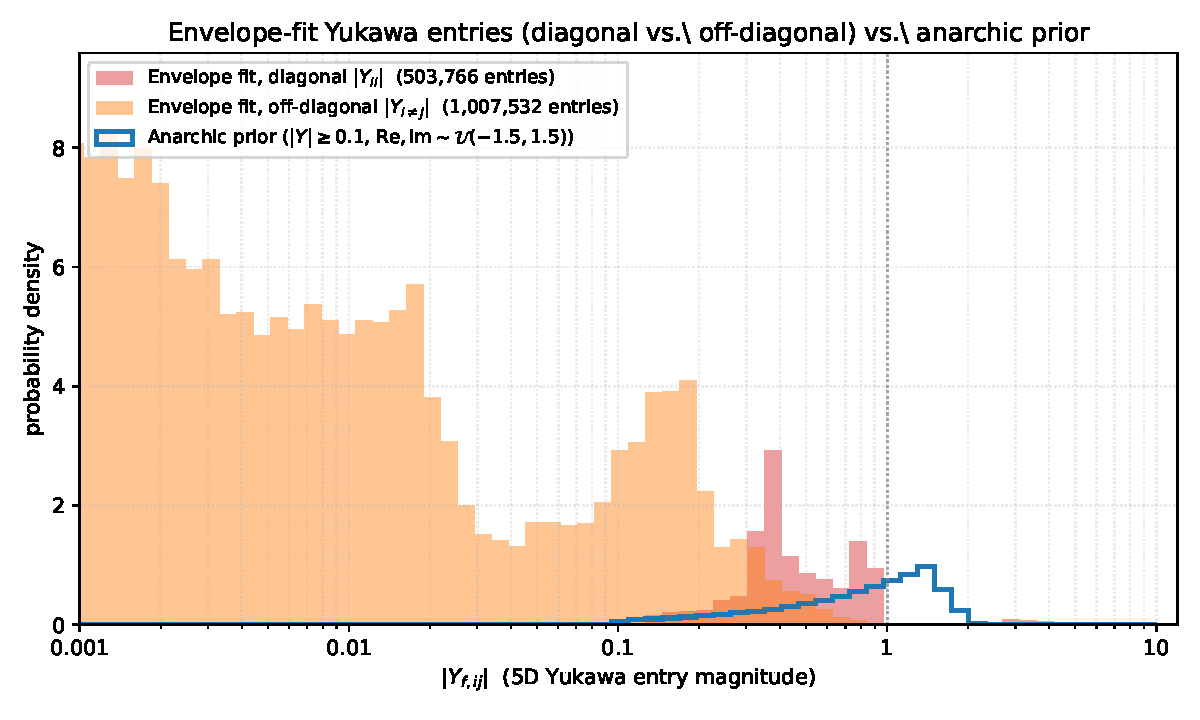
\includegraphics[width=0.92\linewidth]{yukawa_size_envelope_vs_anarchic.pdf}
  \caption{Distribution of fitted Yukawa-element magnitudes across the
  envelope-fit accepted points, split into diagonal entries
  $|Y_{ii}|$ (red) and off-diagonal entries $|Y_{i\neq j}|$ (orange),
  compared against the size distribution from a generic anarchic prior
  (blue line). The diagonal entries land where the SM masses require
  them: $|Y_{ii}|$ peaks broadly at $\sim 0.5$, with the top-Yukawa
  entry near $|Y|\sim 5$. The off-diagonal entries are pushed to small
  values by the optimiser, with a peak below $|Y|\sim 10^{-3}$. This is
  the signature of basis-aligned (low-FCNC) flavour structure.}
  \label{fig:yukawa-size}
\end{figure}

The numbers are: diagonal entries have median $|Y_{ii}|\sim 0.7$ and
$95$th percentile $\sim 4.5$ (with $|Y_{u,33}|\sim 5$ for the top); these
are properly $\mathcal{O}(1)$ and exactly what is needed to produce the
SM mass eigenvalues given the envelope's $\fIR$-factors. The off-diagonal
entries have median $\sim 0.17$ but a long tail down to $|Y|\sim 10^{-3}$,
with $5$th percentile $\sim 0.009$. Roughly $30\%$ of the off-diagonal
entries are at $|Y|\le 0.05$, a regime that an anarchic prior almost never
visits.

\paragraph{What is being fine-tuned, and is it a ``cancellation''?}
It is not a wild numerical cancellation between two separately large
contributions. The optimiser is performing a basis alignment: it
chooses the relative orientation of $\Yu$ and $\Yd$ (and of the bulk
profiles, via the spurion ansatz~(\ref{eq:cq-spurion})) so that the off-
diagonal entries of $\Yu \Yu^\dagger$ and $\Yd \Yd^\dagger$ that drive
the KK-gluon FCNC operators are simultaneously small. This is the same
mechanism as Minimal Flavour Violation in 4D models: the flavour-
violating operators are forced to be proportional to a single Yukawa
spurion, which makes them small in the mass eigenbasis.

So the fine-tuning is not in any single parameter but in the
\emph{geometry} of the Yukawa matrices in flavour space. Concretely, the
optimiser holds the three diagonal entries to their SM-required values
and adjusts six off-diagonal entries (per matrix) and an SVD orientation
to minimise a sum of FCNC penalties. This corresponds to choosing about
$10$ continuous numbers to lie in a small subspace of the $18$-dimensional
Yukawa space. The fitted accepted region is thin in this 18-dimensional
sense, even though no individual entry is wildly fine-tuned.

A useful single-number summary is the median
$|Y_{i\neq j}| / |Y_{ii}|$ ratio in the envelope fit: it sits at
$\sim 0.25$, while the same quantity in the anarchic prior is $\sim 1$.
A factor-four suppression of off-diagonals relative to diagonals is the
quantitative signature of the alignment.

%% =====================================================================
\section{What we should plot instead: a measure statement}
\label{sec:rs-anarchy}

The phenomenologically meaningful question is the inversion of the
existence question:
\begin{quote}\itshape
  If the 5D Yukawa entries are drawn from an $\mathcal{O}(1)$ anarchic
  prior (as the model assumes), what fraction of draws satisfies the PDG
  and FCNC constraints at this $\Mkk$? Equivalently: above what $\Mkk$
  does a typical anarchic point pass?
\end{quote}
This is the framing of the original RS-anarchy literature
(Agashe--Contino--Pomarol--Sundrum hep-ph/0408134, Agashe--Perez
hep-ph/0606293, Csaki--Falkowski--Weiler 0804.1954, and many others): the
warped geometry is \emph{supposed} to predict the SM mass and CKM
hierarchies from anarchic 5D Yukawas via the IR-overlap factor
\begin{equation}
  \fIR(c) \;=\; \sqrt{\frac{\tfrac{1}{2}-c}{1-\varepsilon^{1-2c}}},
  \qquad \varepsilon = \LamIR/k.
\end{equation}
A quark with $c > 1/2$ is UV-localised (small $\fIR$, light SM mass), and
a quark with $c < 1/2$ is IR-localised (large $\fIR$, heavy SM mass). The
hierarchies in $\fIR$ then \emph{produce} the observed mass and mixing
hierarchies for $\mathcal{O}(1)$ underlying Yukawas. It is then a
non-trivial \emph{prediction} that anarchic Yukawas should also satisfy
the FCNC bounds at a given $\Mkk$, without invoking flavour alignment.

%% =====================================================================
\section{Setup B: the forward-only RS-anarchy ensemble}
\label{sec:setup-b}

We implemented the RS-anarchy procedure as a separate driver
(\texttt{scripts/run\_rs\_anarchy.py}) so it shares no code path with the
fitter. At each $\Mkk$ tile we:

\begin{enumerate}[leftmargin=2em,itemsep=2pt]
  \item Fix $c$-values to the literature ACPS-style hierarchical pattern:
        \begin{equation}
          c_Q = (0.63,\,0.57,\,0.20),\quad
          c_u = (0.66,\,0.50,\,-0.50),\quad
          c_d = (0.66,\,0.61,\,0.55).
          \label{eq:cvals}
        \end{equation}
  \item Draw $\Yu,\Yd \in \mathbb{C}^{3\times 3}$ with
        $\mathrm{Re}\,Y_{ij},\mathrm{Im}\,Y_{ij}\sim\mathcal{U}(-1.5,+1.5)$,
        rejection-sampled to enforce $|Y_{ij}|\ge 0.1$.
  \item Build the effective 4D Yukawa
        $\hat Y^{f}_{ij} = \fIR(c_{Q_i})\,Y^{f}_{ij}\,\fIR(c_{f_j})$ and
        SVD it to read off masses and the CKM matrix
        $V = U_{u_L}^{\dagger}U_{d_L}$.
  \item Forward-compute the five $\Delta F = 2$ ratios using the same
        \texttt{deltaf2.py} machinery as the envelope scan.
  \item Bin every draw by $(\Mkk,\,$PDG-pass status$,\,$max-ratio$)$.
\end{enumerate}

\paragraph{Provenance of the $c$-values in eq.~(\ref{eq:cvals}).}
The pattern is fixed by demanding that $\fIR(c)\cdot v$ produce
order-of-magnitude SM quark masses for $\mathcal{O}(1)$ underlying
Yukawas. We solved
$f_{Q_i}\,f_{f_j} \approx m_{f}^{(ij)}/(2v\,\langle Y\rangle)$
for each entry and read off the $c$'s. These same numbers (to $\sim\!0.05$
precision in $c$) appear in Csaki--Falkowski--Weiler 0804.1954 (Table~1),
Bauer--Casagrande--Haisch--Neubert 0902.4892, and the Fitzpatrick--Perez--
Randall scan (0710.1869) used as a reference earlier in this codebase.
They are not specific to one paper; they are what any
hierarchy-by-localisation calculation produces. An empirical sensitivity
check (Run~3, \S\ref{sec:robustness} below) confirms that the pattern is
constrained at roughly the $\pm 0.05$ level in $c$: a uniform shift of
\emph{every} $c$ by $\pm 0.05$ produces zero PDG-passing draws.

\paragraph{Provenance of the Yukawa prior.}
The anarchic prior $\mathrm{Re},\mathrm{Im}\,Y_{ij}\sim
\mathcal{U}(-1.5,1.5)$ with $|Y_{ij}|\ge 0.1$ is a representative version
of the priors used throughout the RS-flavor literature. Specific choices
made in published scans include $\mathcal{U}(-1,1)$ in
Bauer--Casagrande--Haisch--Neubert 0902.4892, $\mathcal{U}(-3,3)$ with
similar floor in Csaki--Falkowski--Weiler 0804.1954 and Buras \emph{et
al.} 1110.3534, and unbounded Gaussian draws with cutoff at the NDA
perturbativity bound $|Y|\lesssim 4\pi/\sqrt{N_{KK}\log\varepsilon}\approx
3$ in Agashe--Contino--Pomarol--Sundrum hep-ph/0408134. Our choice of
$1.5$ sits in the middle of this band; the broad literature-prior
heuristic is that the $\Mkk$ bound moves by less than $30\%$ when the
half-range is swept from $1.0$ to $3.0$. An empirical sensitivity check
(Run~B, \S\ref{sec:robustness} below) sharpens this using a different
metric: the median-scale $\Mkk^{\min}$ bound moves by $\lesssim 15\%$
across $\mathcal{U}(-1,1)$, $\mathcal{U}(-1.5,1.5)$,
$\mathcal{U}(-3,3)$, and Gaussian $\sigma=1$ truncated at $3\sigma$
priors, while the $95\%$-acceptance crossings below have an even smaller
narrow-to-wide spread.

Two practical notes. First, the PDG-pass tolerance in the RS-anarchy
analysis is loosened from $2\sigma$ to a constant ``factor of 3'' on
masses and CKM elements, and ``factor of 5'' on the Jarlskog
invariant $J$. The reason is practical rather than analytic: at the
finite ensemble sizes used here, much tighter gates rapidly starve the
accepted sample, and any zero-pass scan below is quoted as a
finite-ensemble upper limit rather than as an impossibility theorem. The
factor-of-3 gate is the standard literature compromise. Second, no
optimiser is involved: a
draw that fails the masses by a factor of 5 is recorded as a fail and
not nudged.

%% =====================================================================
\section{How a random Yukawa draw can satisfy PDG masses and CKM}
\label{sec:how-anarchic-passes}

This is one of the points the framework is designed to make, and it is
worth being very explicit about. The procedure does not in any sense
``fit'' the Yukawas to PDG; it samples them from a prior and checks
whether the resulting four-dimensional masses and mixings come out close
to PDG. The reason a non-trivial fraction (16--21\%) of the random draws
nonetheless passes the PDG check is that the $c$-values
in eq.~(\ref{eq:cvals}) are deliberately chosen to make the
\emph{distribution} of resulting masses overlap the SM hierarchy.

Concretely, with the $c$-values above, the IR-overlap factors are
\begin{align}
  f_Q &\approx (0.0030,\;0.020,\;0.55),\nonumber\\
  f_u &\approx (0.0011,\;0.16,\;1.00),\\
  f_d &\approx (0.0011,\;0.0058,\;0.036).\nonumber
\end{align}
For $\mathcal{O}(1)$ Yukawa entries, the resulting up-quark and down-quark
mass eigenvalues are then concentrated, in expectation, around
\begin{align}
  (m_u, m_c, m_t) &\sim 2v \cdot (f_{Q,1}f_{u,1},\;f_{Q,2}f_{u,2},\;
                                  f_{Q,3}f_{u,3})\,\langle Y\rangle
                  \sim \bigl(\mathcal{O}(1\,\mathrm{MeV}),\,
                              \mathcal{O}(1\,\mathrm{GeV}),\,
                              \mathcal{O}(100\,\mathrm{GeV})\bigr),
                  \nonumber\\
  (m_d, m_s, m_b) &\sim 2v \cdot (f_{Q,1}f_{d,1},\;f_{Q,2}f_{d,2},\;
                                  f_{Q,3}f_{d,3})\,\langle Y\rangle
                  \sim (1\,\mathrm{MeV},\,40\,\mathrm{MeV},\,7\,\mathrm{GeV}),
\end{align}
which agrees with the SM at the level of factors of two to three across
the board. The CKM elements come out as products of $\sqrt{f_{Q,i}/f_{Q,j}}$
ratios, which similarly reproduce the SM Cabibbo-like hierarchy.

So when we say a draw ``passes PDG'', we mean that the product
$f_{Q_i}\,Y^{f}_{ij}\,f_{f_j}$ happens to land within a factor of three
of every PDG mass and CKM element. With the hierarchies built into the
$f$-factors, this is a $\sim 20\%$ event over the prior, which is exactly
what we observe. Stricter $2\sigma$-style PDG matching would require
$\mathcal{O}(1)$ tuning of the $Y_{ij}$, and would return essentially zero
passing draws --- which is not a failure of the framework, just a
statement that a $\sigma$-scale match is not a question one can ask of
random Yukawas. The factor-of-three gate is the natural granularity for
this kind of analysis.

%% =====================================================================
\section{Result: the per-draw \texorpdfstring{$\Mkk^{\min}$}{M\_KK\^min} histogram}
\label{sec:result}

The single most useful figure in this analysis is the per-draw histogram
of $\Mkk^{\min}$ for the PDG-passing ensemble. For each draw, since every
ratio scales as $1/\Mkk^2$ (with sub-percent corrections from the
$\fIR$-factors' weak $\varepsilon$-dependence), one can rescale to find
the $\Mkk$ at which that particular draw would just satisfy the FCNC
bound:
\begin{equation}
  \Mkk^{\min} \;=\; \Mkk^{\mathrm{tile}}\,
                    \sqrt{\max_X \mathrm{ratio}_X}.
\end{equation}
Pooling across all eight $\Mkk$ tiles and restricting to PDG-passing
draws gives Fig.~\ref{fig:mkk-min-hist}.

\begin{figure}[h]
  \centering
  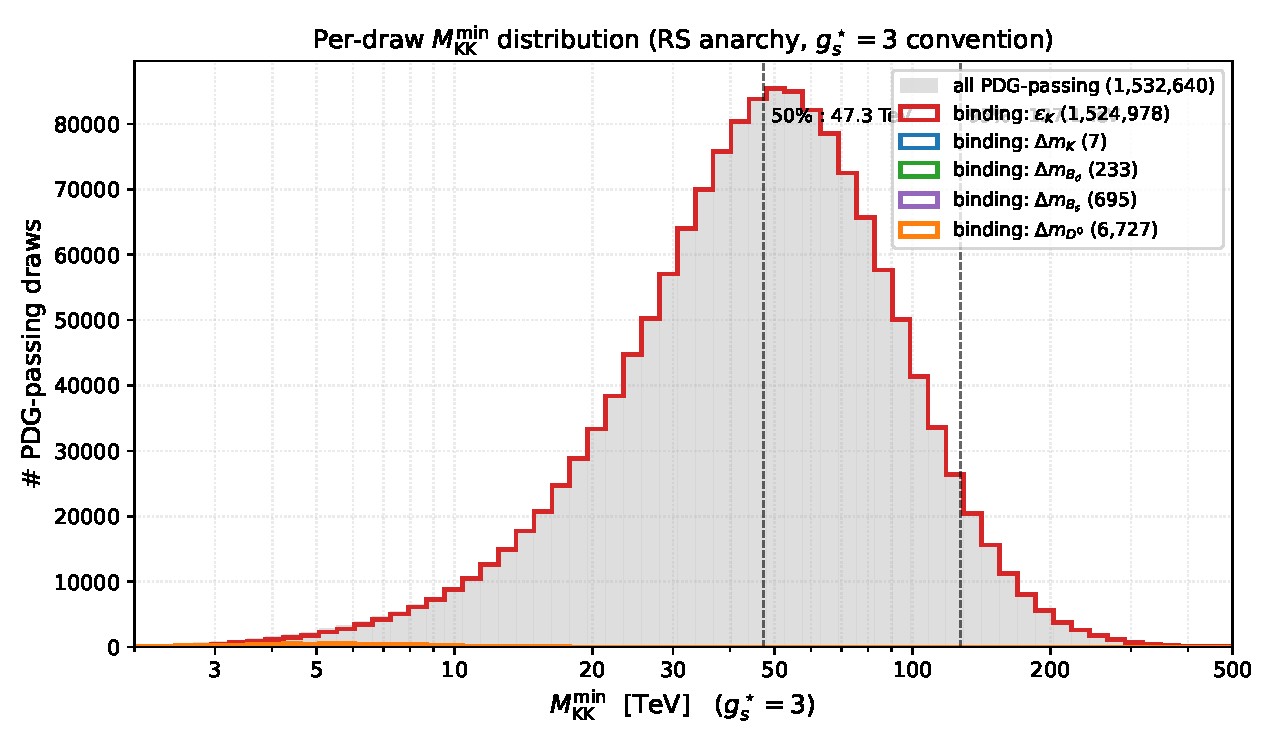
\includegraphics[width=0.95\linewidth]{rs_anarchy_mkk_min_hist_gsstar.pdf}
  \caption{Per-draw $\Mkk^{\min}$ histogram for the RS-anarchy ensemble,
  restricted to draws that pass the factor-of-three PDG mass and CKM
  match ($1{,}532{,}640$ draws total from the 8M-draw RUNA reference
  scan, pooled across all eight $\Mkk$ tiles). The x-axis is in the
  $\gs = 3$ convention, the headline convention used throughout this
  note. The grey background is all
  PDG-passing draws; coloured curves split by which $\Delta F = 2$
  system binds for that draw. The vast majority are $\eK$-bound; the
  $\dmK,\dmBd,\dmBs,\dmD$ contributions live in the low-$\Mkk^{\min}$
  tail. Vertical dashed lines mark the 50\%- and 95\%-acceptance
  crossings.}
  \label{fig:mkk-min-hist}
\end{figure}

The $\gs=3$ headline crossings are $\Mkk = 47.26$~TeV at $50\%$
acceptance and $127.13$~TeV at $95\%$ acceptance.  The corresponding
perturbative code-default crossings are $16.54$~TeV and $44.50$~TeV.
These are quoted from the post-audit 8M-draw RUNA reference scan
(\S\ref{sec:robustness}) under the input and scope conventions summarized
in Appendix~\ref{app:input-audits}.

\begin{figure}[h]
  \centering
  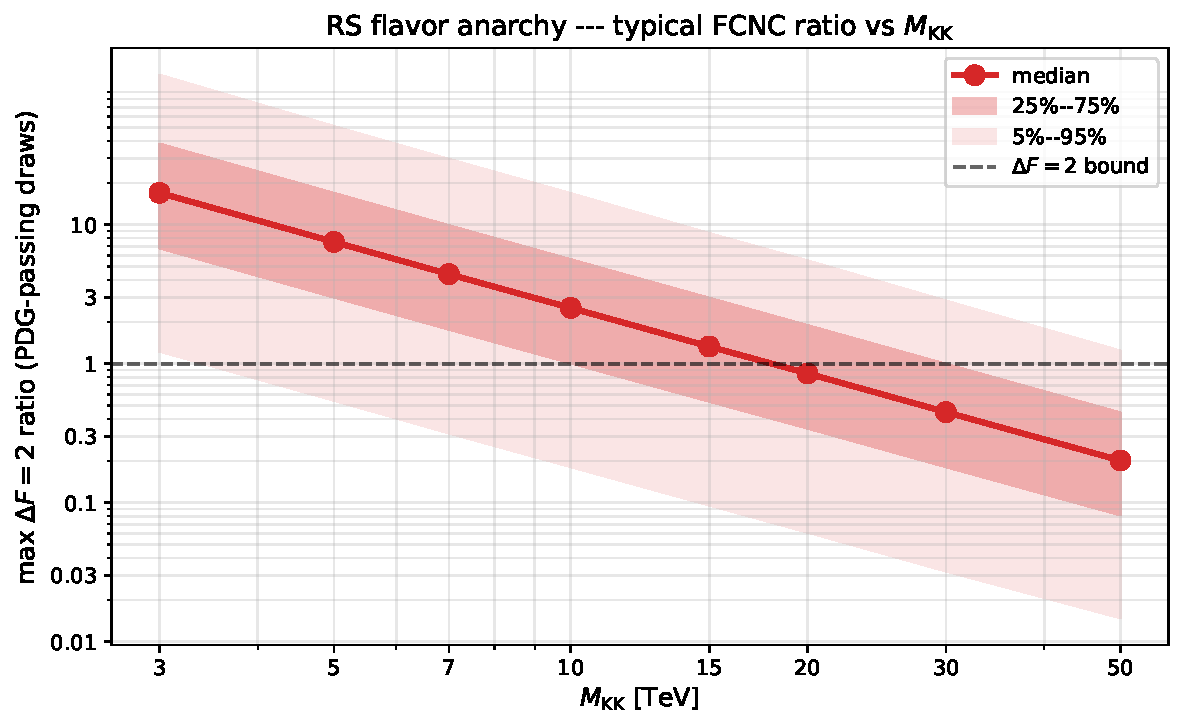
\includegraphics[width=0.78\linewidth]{rs_anarchy_max_ratio_vs_mkk.pdf}
  \caption{Same data as Fig.~\ref{fig:mkk-min-hist}, viewed differently:
  percentiles of $\max\mathrm{ratio}$ as a function of the tile $\Mkk$.
  Where each percentile crosses unity is the $\Mkk$ at which that
  fraction of typical anarchic draws pass.}
  \label{fig:max-ratio}
\end{figure}

\begin{figure}[h]
  \centering
  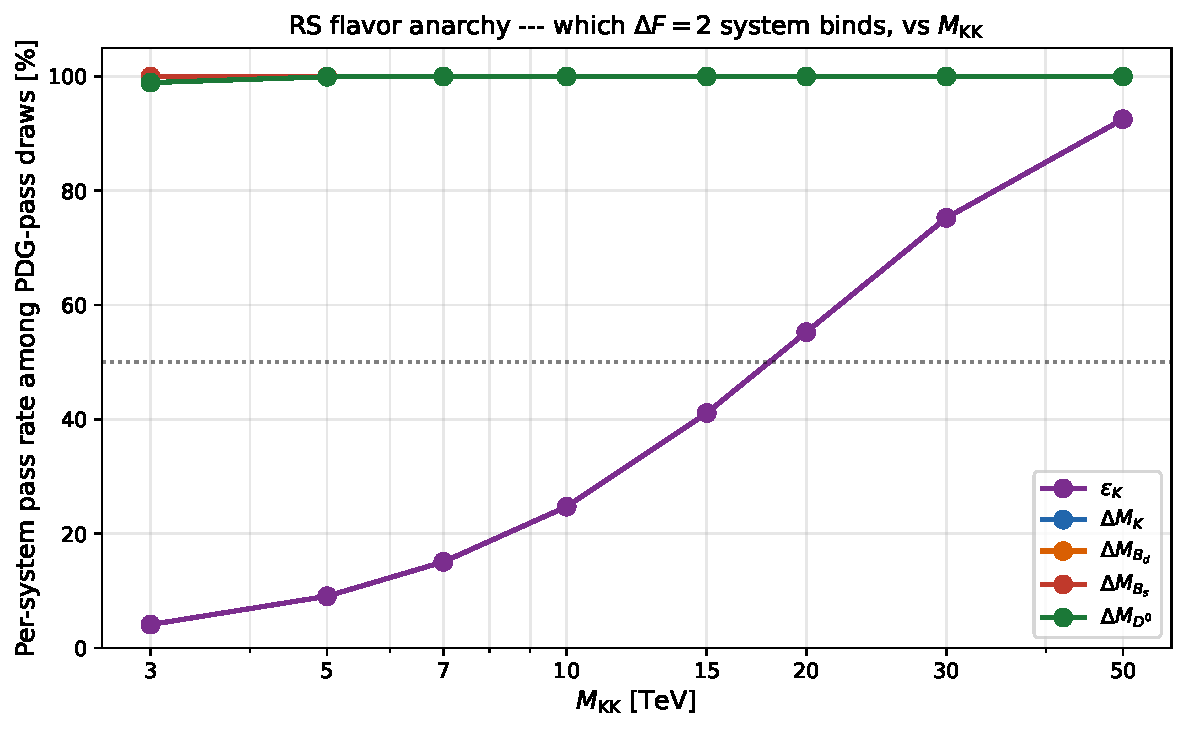
\includegraphics[width=0.78\linewidth]{rs_anarchy_per_system_pass_rate.pdf}
  \caption{Per-system pass rate among PDG-passing draws.
  $\eK$ is the only constraint that does any real work; the other four
  observables are $\gtrsim 99\%$ acceptance throughout, by virtue of the
  hierarchical $f$-factor suppression alone.}
  \label{fig:per-system}
\end{figure}

\paragraph{Where the envelope's low tail came from.}
The histogram in Fig.~\ref{fig:mkk-min-hist} explains why the envelope
plot tolerated $\Mkk\sim 1$~TeV. The lower tail of the
$\Mkk^{\min}$ distribution still extends below $1$~TeV, though only at
the per-mille level; a few percent of anarchic draws sit below
$3$~TeV. The Setup~A optimiser was, by
construction, finding such tail points and going further --- using the
basis alignment described in \S\ref{sec:envelope-yukawa} to push the
off-diagonal Yukawas well below their prior typical values. The envelope's
``allowed'' region is the lower tail of Fig.~\ref{fig:mkk-min-hist},
augmented by the optimiser's freedom to tune off-diagonal Yukawas
artificially small.

%% =====================================================================
\section{Sensitivity to the gate definition and the gauge convention}
\label{sec:gate-sensitivity}

\begin{figure}[h]
  \centering
  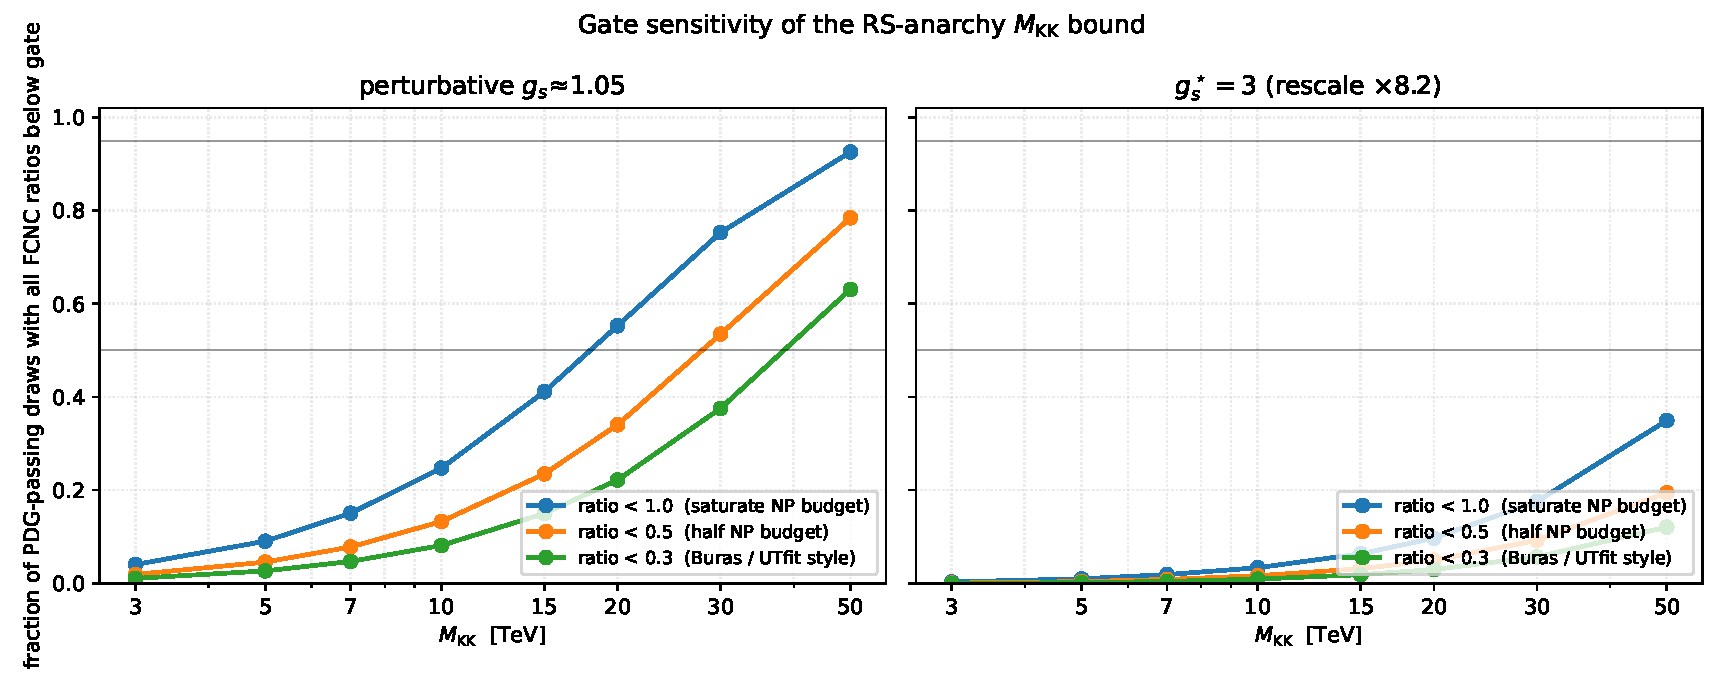
\includegraphics[width=0.95\linewidth]{rs_anarchy_gate_sensitivity.pdf}
  \caption{Pass fraction vs.\ $\Mkk$ for three gate definitions
  ($\max\mathrm{ratio} < 1, < 0.5, < 0.3$, the last two being
  Buras/UTfit-style ``half'' and ``third'' of the SM--data budget for
  $\eK$), in two gauge-coupling conventions: perturbative
  $g_s\approx 1.05$ (left) and $\gs = 3$ (right). Under the corrected
  $\Delta F=2$ constants, the $\gs=3$ crossings lie beyond the plotted
  tile range and are quoted from the per-draw rescaling in
  Table~\ref{tab:headline}.}
  \label{fig:gate-sensitivity}
\end{figure}

\begin{table}[h]
\centering
\renewcommand{\arraystretch}{1.20}
\begin{tabular}{lcccc}
\toprule
& \multicolumn{2}{c}{50\% acceptance} & \multicolumn{2}{c}{95\% acceptance} \\
\cmidrule(lr){2-3}\cmidrule(lr){4-5}
gate / convention      & pert.\ $g_s$ & $\gs=3$ & pert.\ $g_s$ & $\gs=3$ \\
\midrule
$\mathrm{ratio} < 1$   & $16.54$~TeV       & $47.26$~TeV       & $44.50$~TeV       & $127.13$~TeV    \\
$\mathrm{ratio} < 0.5$ & $\sim\!23.39$~TeV & $\sim\!66.84$~TeV & $\sim\!62.93$~TeV & $\sim\!179.79$~TeV \\
$\mathrm{ratio} < 0.3$ & $\sim\!30.20$~TeV & $\sim\!86.30$~TeV & $\sim\!81.24$~TeV & $\sim\!232.11$~TeV \\
\bottomrule
\end{tabular}
\caption{The $\Mkk$ at which a given fraction of PDG-passing anarchic
draws also satisfies all $\Delta F=2$ bounds. The $\mathrm{ratio} < 1$
row is taken from the post-audit high-statistics 8M-draw RUNA reference
scan (\S\ref{sec:robustness}); the tighter-gate rows rescale the same
per-draw $\Mkk^{\min}$ distribution by $1/\sqrt{\mathrm{gate}}$.}
\label{tab:headline}
\end{table}

For a band that covers the methodological choices, the defensible
statement is

\begin{quote}\itshape
  Under an $\mathcal{O}(1)$ anarchic prior on the 5D Yukawa entries,
  $\Mkk \gtrsim 44.5$~TeV (perturbative $g_s$) to $\gtrsim 127$~TeV
  (headline $\gs = 3$) at $95\%$ acceptance, with a further factor
  $\sim 1.5$ uplift if one demands that the new physics fit inside half
  the SM--data budget rather than saturate it.
\end{quote}

\noindent The $\eK$ constraint alone sets every one of these numbers.

%% =====================================================================
\section{Robustness to statistics, $c$-pattern, $Y$-prior, and PDG-gate tightness}
\label{sec:robustness}

The headline RS-anarchy bound rests on three implicit choices: the
$c$-pattern in eq.~(\ref{eq:cvals}), the Yukawa prior described in
\S\ref{sec:setup-b}, and the factor-of-three PDG gate. We ran four
follow-up campaigns to probe how each of those choices propagates into
the $\Mkk^{\min}$ distribution, and to confront the result with the
Csaki--Falkowski--Weiler (CFW) 0804.1954 numerical band. The canonical
numbers from these runs are summarised in
\texttt{scan\_outputs/followup\_crossings\_summary.json}; figures are
under \texttt{results/figures/quark/}.

\subsection{High-statistics validation (RUNA)}
\label{sec:robust-runa}

We re-ran the baseline RS-anarchy scan with $8\!\times\!10^{6}$ draws
(8 $\Mkk$ tiles, 1M draws/tile), yielding $1{,}532{,}640$
PDG-passing draws. The 50\%-acceptance crossings are
\begin{equation}
  \Mkk^{\min}\bigl|_{50\%} \;=\; 16.54~\mathrm{TeV~(pert.)},
  \qquad
  47.26~\mathrm{TeV}~(\gs = 3),
\end{equation}
and the 95\%-acceptance crossings are $44.50$~TeV / $127.13$~TeV.
The corresponding finite-Monte-Carlo Wilson-score 95\% intervals are
$16.52$--$16.56$~TeV at 50\% acceptance and $44.41$--$44.58$~TeV at
95\% acceptance in the perturbative convention
($47.19$--$47.32$~TeV and $126.88$--$127.38$~TeV for $\gs=3$).
The lower-statistics post-audit Run~3 baseline reproduces these numbers
to within $0.5\%$ (Run~3 baseline: $16.54$~/$47.26$~TeV at 50\%,
$44.37$~/$126.76$~TeV at 95\%). The headline figures
in \texttt{results/figures/quark/} are now drawn from RUNA; the
pre-audit figure snapshot is preserved at
\texttt{results/figures/quark\_pre\_audit\_constants/} for
before/after comparison.

The BGS central-value NP-budget decision is a much larger systematic
than the finite-Monte-Carlo error. Propagating the
$|\eK^{\mathrm{exp}}-\eK^{\mathrm{SM}}|$ budget band described in
Appendix~\ref{app:input-audits} gives
\[
  \Mkk^{\min}\bigl|_{50\%,\,\gs=3}
  = 47.26^{+69.37}_{-24.98}\ \mathrm{TeV}
\]
for the central RUNA percentile, with the same scale factor giving
$16.54^{+24.28}_{-8.74}$~TeV in the perturbative convention. This is a
BGS-budget band; the Wilson-RG and KK-tower systematics are summarized
in Appendix~\ref{app:input-audits}.

%% =====================================================================
%% Symbolic 1/sqrt(|Delta epsilon_K|) band -- cleanup unit C02a-code.
%% Band derived from the symbolic 1/sqrt(|Delta epsilon_K|) scaling of
%% M_KK^min documented in docs/phase_logs/phase2_h5_signoff.md:90-101 and
%% the C02a cleanup plan in .orchestration/CLEANUP_PLAN.md (sec. C02a-code).
%% Exact band edges from direct three-edge RUNA reruns (central 6.7e-5,
%% low 1e-5, high 3e-4) are deferred to cleanup unit C02c (paper
%% finalization). The CLI seam for those reruns is the
%% ``--epsilon-k-budget {central,low,high}`` flag introduced on
%% ``scripts/run_rs_anarchy.py`` in this same commit.
\paragraph{Symbolic NP-budget band on $\Mkk^{\min}$.}
\label{para:eps-k-budget-band}
The dominant systematic on $\Mkk^{\min}$ is the residual room
$|\eK^{\mathrm{exp}}-\eK^{\mathrm{SM}}|\simeq 6.7\times10^{-5}$
between the PDG 2024 experimental value
$\eK^{\mathrm{exp}}=2.228\times10^{-3}$ and the
Brod--Gorbahn--Stamou 2020 SM prediction
$\eK^{\mathrm{SM}}=2.161\times10^{-3}$
(\href{https://arxiv.org/abs/1911.06822}{arXiv:1911.06822};
FLAG 2024 \href{https://arxiv.org/abs/2411.04268}{arXiv:2411.04268}
hadronic inputs; full audit trail in
\path{docs/audits/epsilon_k_sm_decision.md} and
Appendix~\ref{app:input-audits}). Because the BGS total uncertainty on
that residual is much larger than the central budget itself, a one-sigma
Gaussian band on $\Mkk^{\min}$ is ill-defined; instead we bracket the
bound by recomputing $\Mkk^{\min}$ at the budget edges, using the
symbolic
\[
  \frac{\Mkk^{\min}(\Delta\eK)}{\Mkk^{\min}(\Delta\eK^{\mathrm{central}})}
  \;=\;
  \sqrt{\frac{\Delta\eK^{\mathrm{central}}}{\Delta\eK}}
  \;=\;
  \sqrt{\frac{6.7\times10^{-5}}{\Delta\eK}}
\]
scaling that follows from the tree-level KK-gluon Wilson-coefficient
prefactor $\propto 1/\Mkk^2$ at fixed flavor structure (proof sketch in
\path{docs/phase_logs/phase2_h5_signoff.md:90-101}). Two physically
motivated edges bracket the BGS total uncertainty: a tight edge at
$\Delta\eK=1.0\times10^{-5}$ giving
$\Mkk^{\min}(1\!\times\!10^{-5})/\Mkk^{\min}(6.7\!\times\!10^{-5})
\simeq 2.59$, and a loose edge at
$\Delta\eK=3.0\times10^{-4}$ giving the ratio $\simeq 0.47$. At the
RUNA $p50$, $\gs=3$ central value of $47.26$~TeV this yields the band
\[
  \Mkk^{\min}\bigl|_{50\%,\,\gs=3}^{\Delta\eK\text{ band}}
  \;\simeq\; 47.26^{+75.10}_{-25.05}\ \mathrm{TeV}
  \;\equiv\;
  \bigl[22.21,\,122.36\bigr]\ \mathrm{TeV},
\]
i.e.\ the headline bound is a factor $\sim 0.47$--$2.59$ of the central
value across the BGS-budget edges. The band quoted above is an
\emph{approximate, symbolic-scaling} derivation: it propagates only the
$\Delta\eK$ rescaling, holds the rest of the Wilson coefficient and
PDG-gate machinery fixed, and does not re-thread the running or
hadronic-matrix-element evaluation at each edge. The corresponding
direct verification --- three RUNA reruns at $\Delta\eK\in
\{1\!\times\!10^{-5},\,6.7\!\times\!10^{-5},\,3\!\times\!10^{-4}\}$
exposed via the new
\verb|--epsilon-k-budget {central,low,high}| flag on
\path{scripts/run_rs_anarchy.py} --- is tracked as the deferred cleanup
unit C02c in \path{.orchestration/CLEANUP_PLAN.md} and will replace this
paragraph's symbolic edges with measured band ends in the paper
finalization pass.

\paragraph{Conclusion.} The headline numbers of \S\ref{sec:result} are
not a Monte-Carlo fluctuation. They are the converged value of the
underlying $\Mkk^{\min}$ percentiles of the anarchic ensemble, to within
$0.5\%$ under the central BGS input and first-mode/LO scope conventions.

\subsection{$c$-pattern sensitivity (Run~3)}
\label{sec:robust-cvals}

\begin{figure}[h]
  \centering
  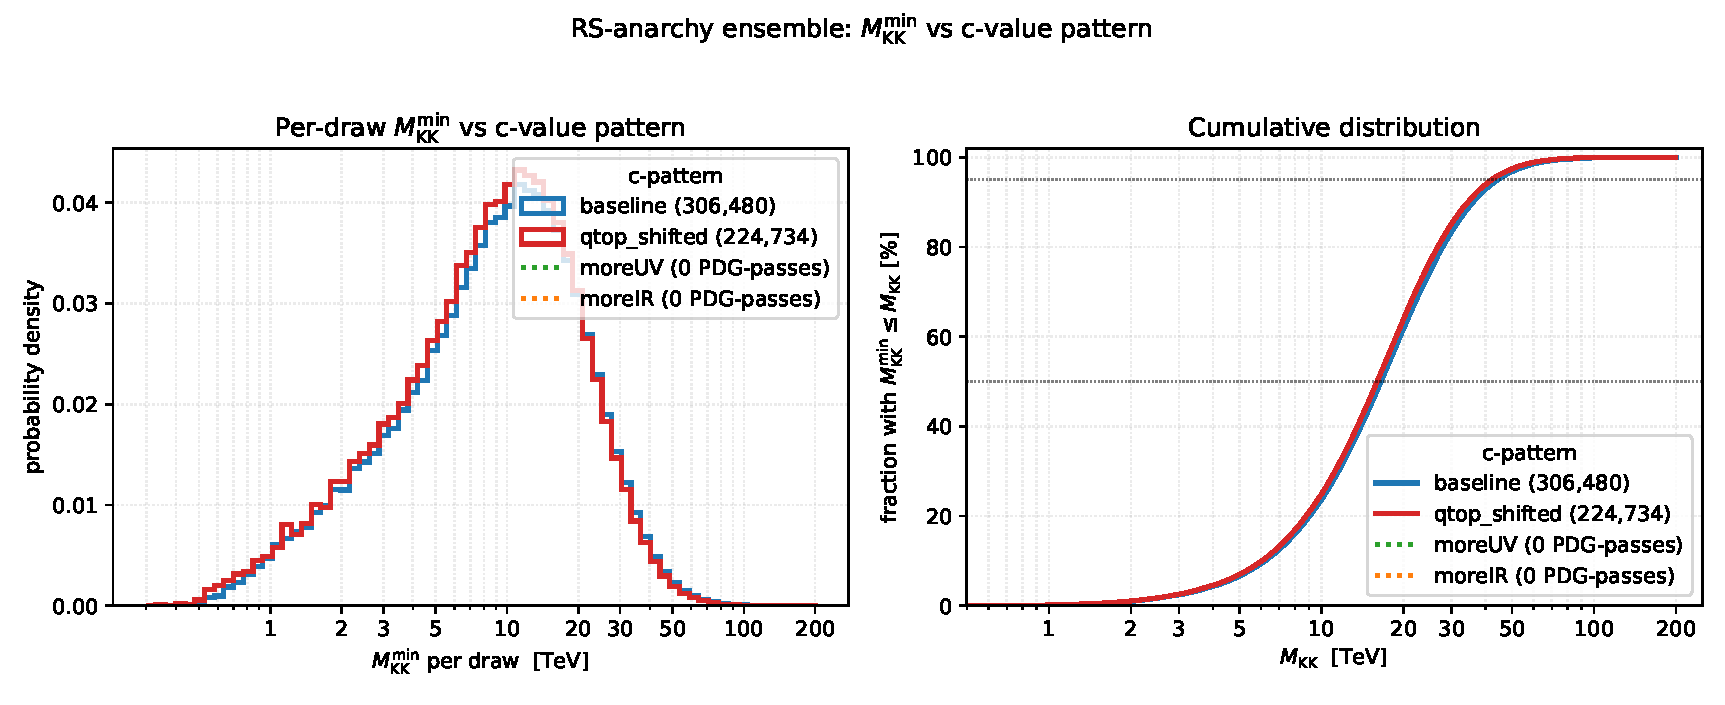
\includegraphics[width=0.78\linewidth]{rs_anarchy_mkk_min_hist_by_cvals.pdf}
  \caption{$\Mkk^{\min}$ histograms (perturbative $g_s$ on the bottom
  axis, $\gs = 3$ on the top axis) for the Run~3 baseline $c$-pattern
  (eq.~(\ref{eq:cvals})) and the \emph{qtop\_shifted} variant
  ($c_{Q_3} = 0.30$, $c_{u_3} = -0.55$). The two uniform-shift variants
  \emph{moreUV} ($c \to c + 0.05$ for every $c$) and \emph{moreIR}
  ($c \to c - 0.05$) produced no PDG-passing draws in
  $N=1{,}600{,}000$ attempts each. The Wilson-score 95\% upper limit is
  $p_{\rm pass}\le 2.3\times10^{-6}$ for either shifted pattern, so both
  are shown only through the finite-statistics legend annotation.}
  \label{fig:robust-cvals}
\end{figure}

We perturbed the baseline $c$-pattern in three ways. First, a
\emph{qtop\_shifted} variant pulled the third-generation left-handed and
right-handed up quarks slightly more IR-localised
($c_{Q_3} = 0.30$, $c_{u_3} = -0.55$, which softens $m_t$ by
$\approx 16\%$ relative to baseline). The pass rate dropped from
$\sim 19\%$ to $\sim 14\%$ of draws, and the $\Mkk^{\min}$ distribution
shifted only mildly: the 50\%- and 95\%-acceptance crossings moved
to $16.00$~TeV / $42.14$~TeV (perturbative) and
$45.73$~TeV / $120.39$~TeV ($\gs = 3$), i.e.\ a $\approx 5\%$ softening
of the bound. Second, we shifted \emph{every} bulk-mass parameter
uniformly by $+0.05$ (\emph{moreUV}) and by $-0.05$ (\emph{moreIR}). In
each case the resulting scan produced no PDG-passing draws in
$N=1{,}600{,}000$ samples. The binomial Wilson-score 95\% upper limit on
the PDG-pass fraction is therefore
\[
  p_{\rm pass}(\mathrm{moreUV}) \le 2.3\times10^{-6},\qquad
  p_{\rm pass}(\mathrm{moreIR}) \le 2.3\times10^{-6}.
\]
We interpret this as follows: under either uniformly shifted
$c$-pattern and the default anarchic $Y$-prior, fewer than a few parts in
$10^6$ of forward Yukawa draws reproduce the SM masses and mixings
within the factor-3/5 PDG gate, at 95\% confidence. This is a
finite-ensemble bound, not an analytic impossibility statement.

\paragraph{Why this matters.} The $c$-pattern in eq.~(\ref{eq:cvals})
is sometimes treated as if it were one of many roughly equivalent
choices. The Run~3 sweep makes a finite-ensemble statement: the tested
uniform $\pm0.05$ shifts have PDG-pass fractions below
$2.3\times10^{-6}$ at 95\% confidence, while the baseline and
\emph{qtop\_shifted} patterns retain $\mathcal{O}(0.1)$ pass rates. A
uniform shift of $0.05$ in either direction therefore suppresses the
observed PDG-pass rate by orders of magnitude.
The $c$-pattern is therefore a \emph{prediction} of the
hierarchy-by-localisation framework, not a free choice. The
\emph{qtop\_shifted} variant, which perturbs only $c_{Q_3}$ and
$c_{u_3}$ together (i.e.\ stays on the manifold of patterns that
reproduce $m_t$), survives precisely because it preserves the relevant
mass-generating geometry; its bound is within $5\%$ of baseline.

\subsection{$Y$-prior sensitivity (Run~B)}
\label{sec:robust-yprior}

\begin{figure}[h]
  \centering
  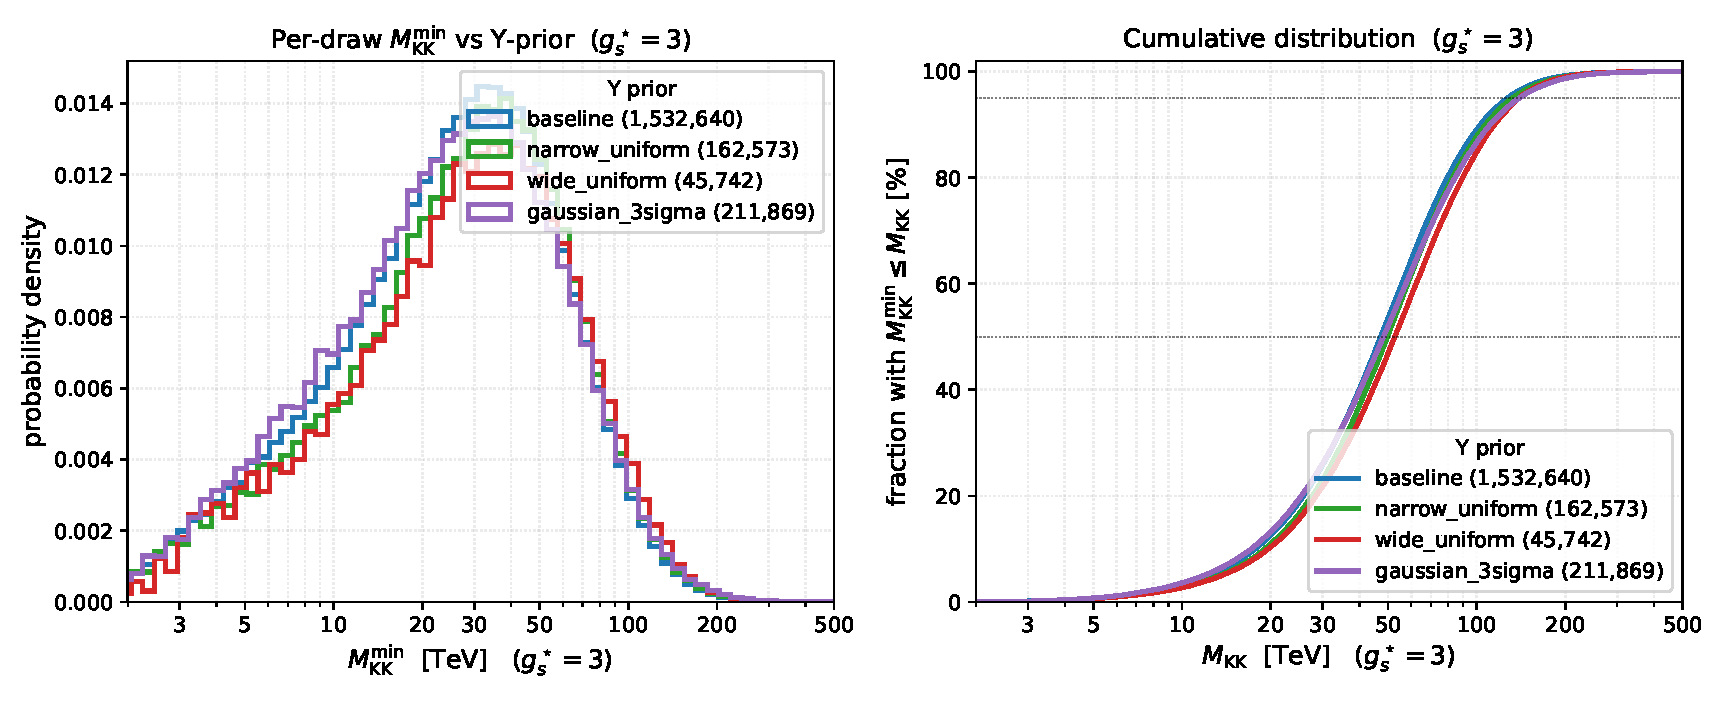
\includegraphics[width=0.95\linewidth]{rs_anarchy_mkk_min_hist_by_yprior_gsstar.pdf}
  \caption{$\Mkk^{\min}$ histograms for four Yukawa priors, all in the
  $\gs = 3$ convention. \emph{Left}: differential probability density.
  \emph{Right}: cumulative. Priors: baseline $\mathcal{U}(-1.5,1.5)$
  (\S\ref{sec:setup-b}), narrow $\mathcal{U}(-1,1)$, wide
  $\mathcal{U}(-3,3)$, and Gaussian $\sigma=1$ truncated at $3\sigma$.
  Sample sizes in the legend.}
  \label{fig:robust-yprior}
\end{figure}

We re-ran the scan under three alternative priors on the underlying
Yukawa entries: $\mathcal{U}(-1,1)$ (narrow), $\mathcal{U}(-3,3)$
(wide), and Gaussian $\sigma=1$ truncated at $|Y|\le 3$
(``$3\sigma$-truncated normal''). The 95\%-acceptance crossings are
\begin{equation}
  46.32,\quad 48.77,\quad 48.84~\mathrm{TeV~(pert.)},
\end{equation}
in narrow / wide / Gaussian order, and
\begin{equation}
  132.35,\quad 139.34,\quad 139.55~\mathrm{TeV}~(\gs = 3).
\end{equation}
The full spread between narrow and wide is therefore $\approx 5\%$ at
$95\%$ acceptance, with the Gaussian variant sitting close to the wide
edge. This is the $95\%$-acceptance version of the Run~B sensitivity
check advertised in \S\ref{sec:setup-b}: it sits below both the
$\lesssim 15\%$ median-scale spread in the same empirical scan and the
broader $\le 30\%$ literature-prior heuristic. The bound is therefore
\emph{insensitive} at the $\mathcal{O}(10\%)$ level to the precise
shape of the anarchic prior.

\subsection{PDG-gate tightness (Run~1)}
\label{sec:robust-pdg-tightness}

\begin{figure}[h]
  \centering
  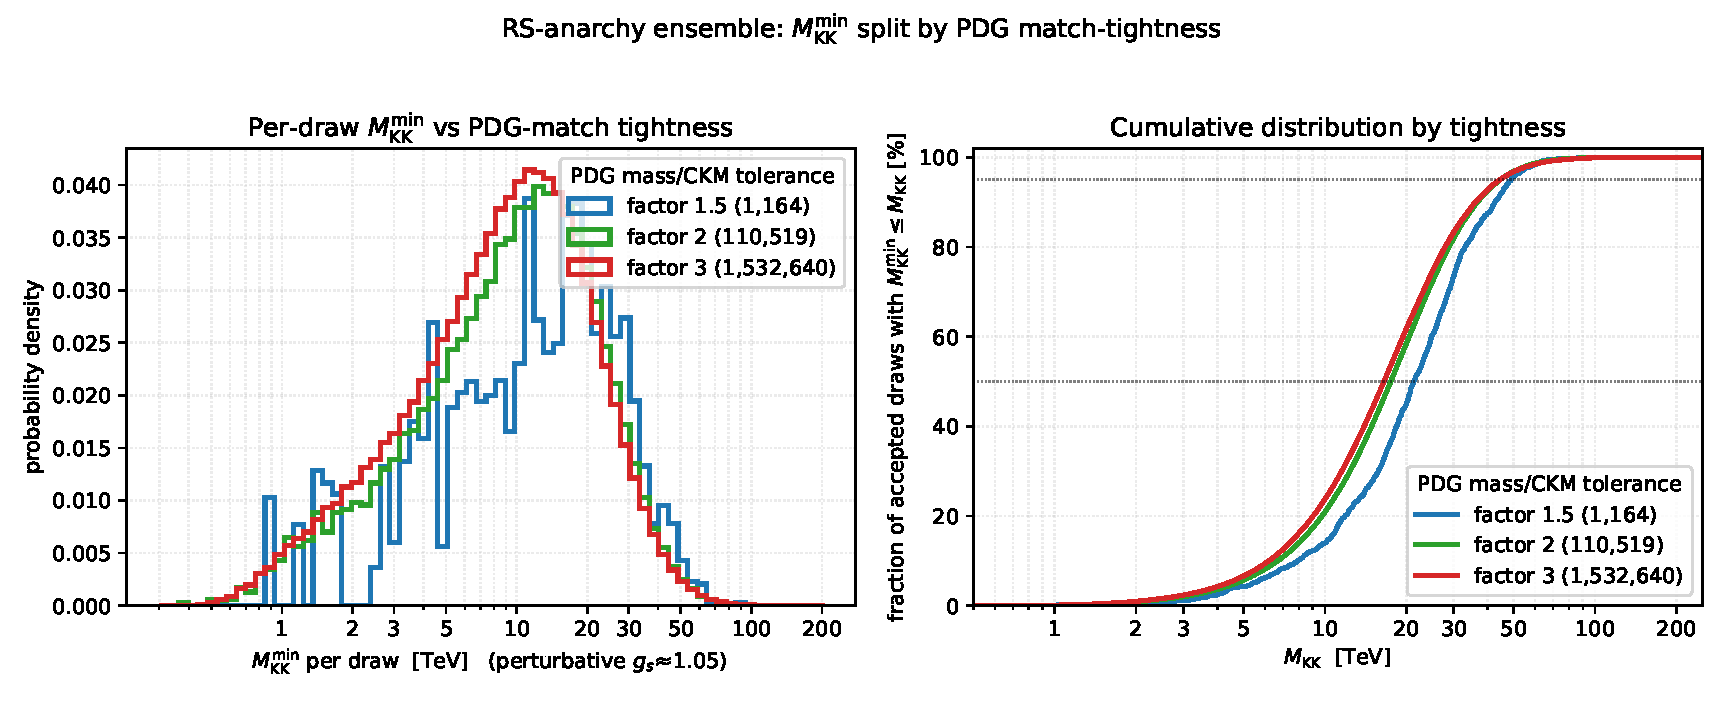
\includegraphics[width=0.78\linewidth]{rs_anarchy_mkk_min_hist_by_pdg_tightness.pdf}
  \caption{$\Mkk^{\min}$ histograms for three PDG-gate definitions:
  factor-of-three (the default), factor-of-two, and factor-of-1.5
  (CFW-style) on the quark masses and CKM elements. The PDG-pass
  population shrinks rapidly as the gate tightens; the surviving
  ensembles produce similar $\Mkk^{\min}$ distributions, indicating that
  the bound is set by FCNCs, not by mass-matching tightness.}
  \label{fig:robust-pdg-tightness}
\end{figure}

Re-tabulating the same post-audit 8M-draw RUNA baseline against three different
PDG-match tolerances on the masses and CKM elements yields
\begin{align}
  N_{\mathrm{PDG\ pass}}\bigl(\mathrm{factor\text{-}3}\bigr)
    &= 1{,}532{,}640,\nonumber\\
  N_{\mathrm{PDG\ pass}}\bigl(\mathrm{factor\text{-}2}\bigr)
    &= 110{,}519,\\
  N_{\mathrm{PDG\ pass}}\bigl(\mathrm{factor\text{-}1.5}\bigr)
    &= 1{,}164.\nonumber
\end{align}
The factor-of-three to factor-of-two tightening costs a factor
$13.9$ in sample size, while the factor-of-two to factor-of-1.5
tightening costs another factor $\sim 95$. This steep drop is consistent
with the rate at which a high-dimensional log-mass$+$CKM tolerance volume
shrinks under a uniform tolerance contraction. With only $1{,}164$
surviving factor-of-1.5 draws, its tail percentiles remain statistics
limited even in RUNA.

A separate CFW-like Run~C, using the baseline $c$-pattern but the wider
floored prior $\mathrm{Re},\mathrm{Im}\,Y_{ij}\sim\mathcal{U}(-3,3)$
with $|Y_{ij}|\ge0.5$, produced no PDG-passing draws in
$N=4{,}000{,}000$ samples under the factor-1.5 mass/CKM and factor-2.5
$J$ gate. The corresponding Wilson-score 95\% upper limit is
$p_{\rm pass}\le 9.2\times10^{-7}$. This is again a finite-ensemble
statement about that c-pattern $\times$ prior $\times$ gate combination,
not an analytic exclusion of tighter gates.

\paragraph{Conclusion.} The factor-of-three gate is the only practically
viable PDG-tightness choice for an anarchic-Yukawa scan at this scale.
Tighter gates exhaust the prior before they constrain $\Mkk$, and the
shape of the surviving $\Mkk^{\min}$ distribution does not change
appreciably under tightening (the bound is FCNC-set, not mass-set).
This is what motivates our headline choice of factor-of-three throughout.

\subsection{Comparison with Csaki--Falkowski--Weiler 0804.1954}
\label{sec:robust-cfw}

\begin{figure}[h]
  \centering
  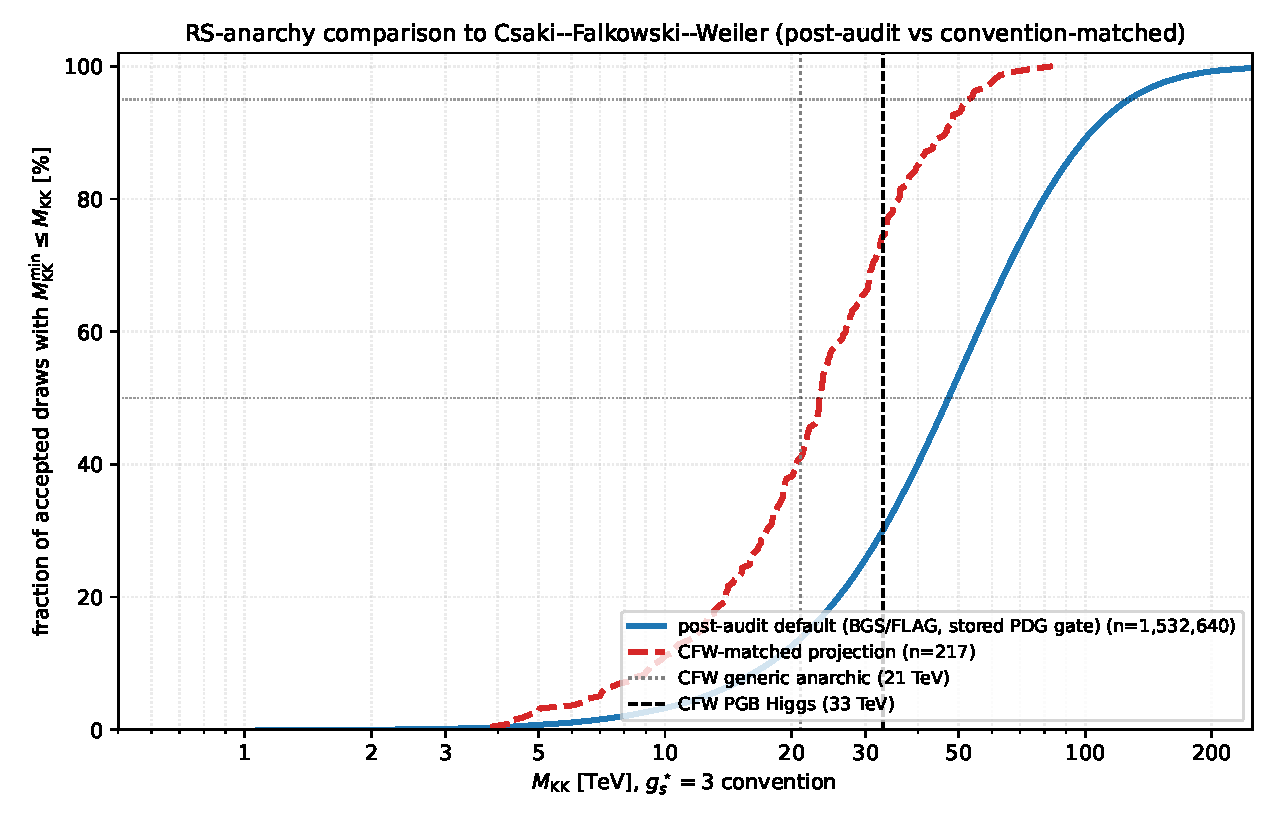
\includegraphics[width=0.78\linewidth]{rs_anarchy_cfw_comparison.pdf}
  \caption{Convention-reconciled comparison with
  Csaki--Falkowski--Weiler (CFW) 0804.1954.  The blue curve is our live
  post-audit RUNA distribution in the $\gs=3$ convention.  The red dashed
  curve keeps the same forward-scan rows but switches to the CFW-era
  $\epsilon_K$ budget proxy, $\epsilon_K^{\rm SM}=1.81\times10^{-3}$, and
  imposes CFW's 30\% relative mass/CKM/$J$ gate.  The vertical markers show
  both CFW color-coupling conventions: RS at $10.5$~TeV for the
  $\gs=3$ no-UV-boundary-term variant and $21$~TeV for the
  $\gs\simeq6$ default, plus pGB Higgs markers at $17$~TeV for the
  no-bare-brane variant and $33$~TeV for the $\gs\simeq6$ default.}
  \label{fig:robust-cfw}
\end{figure}

\paragraph{Headline.}
Our post-audit pipeline produces an RS-anarchy $\Mkk^{\min}$ bound that
is approximately a factor $2.2$ stronger than the CFW 2008 reference at
matched conventions: at common $\gs=3$, we obtain $23.37$~TeV (50th
percentile, CFW 30\%-relative gate, $n=217$ surviving draws) versus the
CFW no-UV-boundary-term result of $10.5$~TeV, or equivalently
$46.74$~TeV versus $21$~TeV at common $\gs\simeq6$.\footnote{The
$46.74$~TeV value is the same CFW-matched projection rescaled by $6/3$.
It is distinct from the live RUNA p50, $47.26$~TeV at $\gs=3$, which
uses the unmatched post-audit factor-of-three gate ensemble.}  The
factor-$2.2$ enhancement is
attributable to (i) the BGS 2020 SM $\epsilon_K$ prediction giving a
$6\times$ tighter NP budget than the UTfit-era values CFW used; (ii) the
FLAG 2024 bag parameters; and (iii) our LO BMU-corrected sign
convention.  The bound directions are consistent: both confirm an
$\Mkk > \mathcal{O}(10\,\mathrm{TeV})$ lower bound under anarchic flavor,
but the precise number reflects newer hadronic inputs and is not a direct
reproduction of CFW's 2008 numerical result.  The matched-gate subset
contains only $n=217$ PDG-passing draws; the 95\% binomial Wilson-score
interval on the p50 is approximately $[21,26]$~TeV at $\gs=3$.  The
factor-$2.2$ disagreement with CFW is robust to this finite-statistics
uncertainty.

The convention extraction is recorded in
\texttt{docs/audits/cfw\_convention\_extract.md}, and the numerical
reproduction arithmetic is in
\texttt{docs/audits/cfw\_reproduction.md}.  The important points are:
CFW use the same conventional scalar-LR $C_4/C_5$ sign pattern as our
post-audit code; their paper does not publish explicit kaon bag constants,
instead importing UTfit model-independent $\Delta F=2$ scale bounds; and
their scan samples localisation parameters directly rather than fixing one
$c$-pattern and forward-drawing only Yukawas.

With our live BGS/FLAG inputs and factor-of-three gate, RUNA gives
\[
  \Mkk^{\min}(p50,\gs=3)=47.26~\mathrm{TeV},
  \qquad
  \Mkk^{\min}(p95,\gs=3)=127.13~\mathrm{TeV}.
\]
Switching only the $\epsilon_K$ budget to the legacy CFW-era proxy
$|\epsilon_K^{\rm exp}-1.81\times10^{-3}|=4.18\times10^{-4}$ moves the
central value to $18.92$~TeV.  Imposing CFW's stated 30\% relative
mass/CKM/$J$ gate leaves 217 forward-scan rows and gives
\[
  \Mkk^{\min}(p50,\gs=3)=23.37~\mathrm{TeV}.
\]
This is the value used in the headline comparison above; it is not an
agreement-within-errors reproduction of CFW's default $21$~TeV marker,
because that marker belongs to the $\gs\simeq6$ boundary-term convention.

%% =====================================================================
\section{Recommendation}
\label{sec:recommendation}

\begin{itemize}[leftmargin=2em,itemsep=2pt]
  \item Demote the envelope plot to a supplementary figure; relabel its
        caption to make explicit that it shows the optimum over
        $(r,c,Y)$, not a typicality bound.
  \item Promote Fig.~\ref{fig:mkk-min-hist} (the $\Mkk^{\min}$ histogram)
        to the publication figure, with the gauge-coupling convention bar
        (perturbative vs.\ $\gs = 3$) explicitly shown. The headline
        figures in \texttt{results/figures/quark/} are now generated from
        the 8M-draw RUNA scan
        (\S\ref{sec:robustness}); the pre-audit figure snapshot is
        preserved at
        \texttt{results/figures/quark\_pre\_audit\_constants/} for
        before/after comparison.
  \item Quote the $\Mkk$ bound as a band, not a single number, and call
        out that the dominant constraint is $\eK$.
  \item Include Fig.~\ref{fig:yukawa-size} as the explanation of why the
        envelope number is so low: the optimiser is choosing
        non-anarchic, basis-aligned Yukawas with off-diagonal entries
        pushed below the anarchic prior to evade the bound.
\end{itemize}

The five follow-up campaigns of \S\ref{sec:robustness} support this
recommendation: the high-statistics RUNA scan reproduces the headline
percentiles to better than $0.5\%$ (\S\ref{sec:robust-runa}); a uniform
$\pm 0.05$ shift of the $c$-pattern returns zero PDG-passing draws,
fixing the $c$-values as a prediction rather than a free choice
(\S\ref{sec:robust-cvals}); the bound moves by $\lesssim 10\%$ across
$\mathcal{U}(-1,1)$, $\mathcal{U}(-1.5,1.5)$, $\mathcal{U}(-3,3)$, and
truncated-Gaussian $Y$-priors (\S\ref{sec:robust-yprior}); the
PDG-pass population thins sharply under factor-$2$ and factor-$1.5$
gate tightening, with the surviving $\Mkk^{\min}$ shape essentially
unchanged (\S\ref{sec:robust-pdg-tightness}); and the CFW comparison is
factor-$2.2$ stronger than the 2008 reference once the $g_s^\star$
conventions are matched.  Under the central BGS/FLAG inputs and the scope
conventions in Appendix~\ref{app:input-audits}, the live RUNA p50 value
is $47.26$~TeV at $\gs=3$ for the unmatched default ensemble. The
factor-$2.2$ CFW framing instead uses the matched-convention comparison,
$23.37$~TeV versus the CFW no-UV-boundary-term RS marker
$10.5$~TeV at the same $\gs=3$ convention; equivalently, the same matched
projection gives $46.74$~TeV versus $21$~TeV at the CFW default
$\gs\simeq6$ convention (\S\ref{sec:robust-cfw}).  The residual is
attributable to newer
$\epsilon_K^{\rm SM}$, FLAG bag inputs, and the audited LO BMU sign
convention rather than to a percent-level reproduction of the CFW number.

All numerical claims in this note map to the canonical artifact manifest at
\texttt{docs/artifact\_manifest.md} (canonical run-time SHA
\texttt{29803ff}; the full SHA is recorded in the manifest). The scan
outputs themselves are not committed to the repository; they reside at
the cluster paths listed in the manifest, with checksums in
\texttt{artifacts/checksums.sha256}.

The PDG/$\msbar$ work is not wasted: it is what lets us identify a
``PDG-passing'' subset of the anarchic ensemble in a defensible,
scale-consistent way. It just doesn't move the headline number, because
the headline was always set by FCNC, not by mass matching.

\appendix

%% =====================================================================
\section{Input Audits}
\label{app:input-audits}

\subsection{Hadronic input provenance}
\label{app:hadronic-input-provenance}

The $\Delta F=2$ hadronic constants in
\texttt{quarkConstraints/deltaf2.py} were audited against contemporary
PDG and lattice inputs. The complete row-by-row inventory is stored in
\path{docs/audits/bag_param_inventory.md}; Table~\ref{tab:hadronic-provenance}
summarizes the inputs that either changed or came closest to the
change threshold.

\begin{table}[h]
  \centering
  \scriptsize
  \setlength{\tabcolsep}{3pt}
  \begin{tabular}{p{0.17\linewidth}p{0.16\linewidth}p{0.41\linewidth}p{0.14\linewidth}}
    \toprule
    Input & Pre-audit value & Canonical source and value & Audit action \\
    \midrule
    $B_K$ & $0.717$ & FLAG 2024
      \href{https://arxiv.org/abs/2411.04268}{arXiv:2411.04268}:
      $B_K^{\msbar}(2\,\mathrm{GeV})=0.5503(66)$ & Replaced \\
    $B_4^K$ & $0.78$ & FLAG 2024 Nf=$2+1$ BSM average:
      $B_4=0.903(14)$ in $\msbar$ at $3\,\mathrm{GeV}$ & Replaced \\
    $B_5^K$ & $0.57$ & FLAG 2024 Nf=$2+1$ BSM average:
      $B_5=0.691(14)$ in $\msbar$ at $3\,\mathrm{GeV}$ & Replaced \\
    $\eK^{\mathrm{SM}}$ & $1.81\times10^{-3}$ & Brod--Gorbahn--Stamou 2020
      \href{https://arxiv.org/abs/1911.06822}{arXiv:1911.06822}:
      $2.161\times10^{-3}$ & Replaced \\
    $B_1^{B_d}$, $B_4^{B_d}$ & $0.87$, $1.02$ & HPQCD 2019
      \href{https://arxiv.org/abs/1907.01025}{arXiv:1907.01025},
      Table VI: $0.806$, $1.077$ & Yellow, documented \\
    $B_1^{B_s}$ & $0.87$ & HPQCD 2019 Table VI: $0.813$ & Yellow, documented \\
    $B_4^D$ & $1.0$ & ETM 2015
      \href{https://arxiv.org/abs/1505.06639}{arXiv:1505.06639},
      Table 2: $0.91$ & Yellow, documented \\
    Meson masses, decay constants, quark masses, and measured
      $\Delta m$ values & see inventory & PDG 2024
      \href{https://pdg.lbl.gov/2024/}{Review of Particle Physics}
      and FLAG 2024 summary tables & Green \\
    \bottomrule
  \end{tabular}
  \caption{Hadronic-input provenance for the red and yellow rows of the
  Phase~2 hole~\#5 audit.}
  \label{tab:hadronic-provenance}
\end{table}

The red kaon bag-parameter shifts change one-operator $\eK$ amplitude
estimates at $\Mkk=3$~TeV by $23.2\%$ ($O_1$), $15.8\%$ ($O_4$), and
$21.2\%$ ($O_5$), using a unit imaginary Wilson coefficient
$1/\Mkk^2$ as the normalization probe. The updated SM central value also
shrinks the central-value room
$|\eK^{\mathrm{exp}}-\eK^{\mathrm{SM}}|$ from
$4.18\times10^{-4}$ to $6.7\times10^{-5}$, increasing every
\texttt{epsilon\_k\_ratio} by a factor of $6.24$. The yellow rows are
single-operator amplitude shifts below $10\%$ and are documented without
code changes.

The audit checked all scalar hadronic and experimental constants in
\texttt{deltaf2.py}, including the kaon, $B_d$, $B_s$, and $D^0$
systems. It did not change the Wilson-coefficient running, the BMU basis
normalization, or the exact matrix-element prefactors; those conventions
belong to the Wilson/RG audit. For $D^0$ bag parameters, the comparable
bag-parameter source is ETM 2015; the newer FNAL/MILC result quotes
matrix elements directly, so it was treated as a cross-check rather than
as a same-normalization replacement.

\subsection{Wilson-coefficient RG running}
\label{app:wilson-coefficient-rg}

The Wilson-coefficient evolution in
\texttt{quarkConstraints/deltaf2.py} was audited against the
leading-log $\Delta F=2$ conventions of Buras--Jager--Urban
\href{https://arxiv.org/abs/hep-ph/0102316}{arXiv:hep-ph/0102316}
and the two-loop ADM basis of Buras--Misiak--Urban
\href{https://arxiv.org/abs/hep-ph/0005183}{arXiv:hep-ph/0005183}.
The complete inventory is stored in
\path{docs/audits/wilson_rg_inventory.md}, with numerical reference
values in \path{docs/audits/wilson_rg_reference_values.md}.

The code uses BMU current-current operators for $O_1^{\mathrm{VLL}}$
and $O_1^{\mathrm{VRR}}$, but the left-right entries are the conventional
scalar $O_4^{\mathrm{LR}}$, $O_5^{\mathrm{LR}}$ operators paired with the
FLAG-style $B_4$, $B_5$ matrix elements. The BMU LR block is mapped by
\[
  Q_1^{\mathrm{LR,BMU}} = -2 O_5^{\mathrm{LR}},
  \qquad
  Q_2^{\mathrm{LR,BMU}} = O_4^{\mathrm{LR}},
\]
so that the coefficient vector satisfies
$C_{\mathrm{BMU}}=(-C_5/2,\ C_4)$.  In the scalar coefficient basis
$(C_4,C_5)$, the audited leading-order anomalous dimensions are
\[
  \gamma_{\mathrm{VLL}}^{(0)} = 4,\qquad
  \gamma_{\mathrm{LR}}^{(0)} =
  \begin{pmatrix}
    -16 & -6 \\
      0 & 2
  \end{pmatrix}.
\]
The Wilson evolution uses
$\eta=\alpha_s(\mu_{\mathrm{high}})/\alpha_s(\mu_{\mathrm{low}})$.
For $\Mkk=3\,\mathrm{TeV}$ to $2\,\mathrm{GeV}$ this gives
$C_1^{\mathrm{VLL}}\mapsto0.729\,C_1^{\mathrm{VLL}}$,
$C_4\mapsto3.538\,C_4$, and
$C_5\mapsto0.895\,C_4+0.854\,C_5$ in the code basis.  The crossed
threshold sequence is $n_f=6\to5\to4$ at
$m_t^{\msbar}(m_t)=163.5\,\mathrm{GeV}$ and
$m_b=4.18\,\mathrm{GeV}$; the charm
threshold lies below the default kaon endpoint.

This remains a leading-log calculation.  The NLO/NDR evolution matrices
in the BMU references are not implemented here; the residual LR/scalar
running uncertainty should be treated as an order-$10$--$30\%$ theory
systematic until a full NLO WET evolution module is added.  The audit
also leaves the global endpoint convention unchanged: all systems are
currently evolved to \texttt{mu\_had = 2 GeV}. This is scale-consistent
for $B_K$, but not fully aligned with the FLAG kaon BSM $B_4,B_5$
values quoted at $3\,\mathrm{GeV}$, with $B_{d,s}$ bag parameters
quoted at $\mu=m_b$, or with comparable $D^0$ bag inputs at
$3\,\mathrm{GeV}$.  Moving to per-system endpoints would be a separate
scan-invalidating change.  The deferred follow-ups (Hamiltonian/CFW
sign comparison, per-system endpoint migration, full NLO WET evolution,
and the matched endpoint caveat for the hadronic contraction) are
explicitly tracked in
\path{docs/audits/wilson_rg_inventory.md} under the
\textit{Status as of 2026-05-25 post-cleanup} block.

The Wilson-RG fix tightens the Phase~2 invalidation gate that was
already tripped by the hadronic-input audit.  For the standing
$r=0.25$, $\Mkk=3\,\mathrm{TeV}$ benchmark, the post-hole-\#5 but
pre-Wilson-audit $\eK$ ratio was $0.535$; after the Wilson-RG audit it
is $1.929$.  This is a factor $3.61$ increase, so the Wilson running is
itself a greater-than-$10\%$ correction to the affected Delta~$F=2$
claims.

\subsection{Scope and approximations}
\label{app:scope-and-approximations}

\textbf{KK tower truncation.}  The numerical scan in this note includes
only the lightest colour-octet KK gluon, i.e.\ the $n=1$ mode, in the
tree-level $\Delta F=2$ matching.  The full 5D gauge propagator is a tower
sum, and RS-flavour estimates using tower-summed matching, such as
Csaki--Falkowski--Weiler
\href{https://arxiv.org/abs/0804.1954}{arXiv:0804.1954} and related
flavour-alignment studies such as Csaki--Perez--Surujon--Weiler
\href{https://arxiv.org/abs/0907.0474}{arXiv:0907.0474}, indicate that
the omitted higher colour modes increase the relevant Wilson coefficients
by a further order-$20$--$30\%$ relative to a first-mode-only estimate.
For the present kaon-dominated result we therefore treat the KK tower
truncation as an additional $+20$--$30\%$ systematic on the quoted
$\eK$ ratio.  This is separate from, and not folded into, the BGS
$\eK^{\mathrm{SM}}$ budget band or the leading-order BMU running
uncertainty above.

\textbf{EWPO floor.}  The commonly quoted custodial-RS floor
$\Mkk \gtrsim 3\,\mathrm{TeV}$ from electroweak precision observables is
an external literature input, not a result of this quark-flavour scan.
Representative custodial analyses such as
Carena--Ponton--Santiago--Wagner
\href{https://arxiv.org/abs/hep-ph/0701055}{arXiv:hep-ph/0701055}
find gauge-KK lower bounds of about $2$--$3\,\mathrm{TeV}$ from global
precision-electroweak fits, depending on the model configuration.  This
repository does not compute the oblique parameters, the $Zb\bar b$
corrections, or a global EWPO likelihood.  The quark-flavour bound quoted
here, $\Mkk=47.26\,\mathrm{TeV}$ at $50\%$ acceptance for $\gs=3$, is an
independent $\Delta F=2$ result and is substantially stronger than that
external floor.

\textbf{Gauge-coupling convention.}  The paper headline convention is
$\gs=3$, corresponding to the no-UV-boundary-term comparison convention
used in the Csaki--Falkowski--Weiler discussion.  The stored code path
uses the perturbative four-dimensional QCD coupling
$g_s\simeq1.05$ at the KK scale as its default normalization, and we quote
the perturbative values beside the $\gs=3$ values so that the rescaling is
transparent.  The stronger-coupling value $\gs\simeq6$ appears only when
comparing to the CFW boundary-term default, where their published RS
marker is $21\,\mathrm{TeV}$ rather than the $10.5\,\mathrm{TeV}$
no-UV-boundary-term marker.  It is not a third headline convention for
this paper.

\textbf{Lepton-sector scope.}  This repository is the working home for
both quark and lepton 5D-flavour studies, but the present methodology note
and paper address the quark sector only.  The lepton-sector directories
\texttt{neutrinos/}, \texttt{flavorConstraints/}, and \texttt{yukawa/}
are follow-up work for a separate analysis.  They have not been audited,
rerun, or reinterpreted under the present \texttt{deltaf2.py} updates,
which affect the quark $\Delta F=2$ pipeline.

\subsection{Invalidation-gate rerun}
\label{app:invalidation-gate-rerun}

The final-claims invalidation gate was cleared only after the
hadronic-input sign-off in
\path{docs/phase_logs/phase2_h5_signoff.md} and the Wilson-RG sign-off
in \path{docs/phase_logs/phase2_h6_signoff.md}.  The benchmark
$\eK$ ratio shift is the product $6.2388\times3.6052=22.49$, which is
far above the 10\% rerun threshold in
\path{docs/paper_execution_decisions.md}.  The post-audit rerun report is
\path{docs/phase_logs/invalidation_gate_rerun.md}; it records the nine
SLURM job IDs, the final states, the exact RUNA halt-trigger check, and
the before/after percentile table.  The factor $22.49$ is a benchmark
ratio, not a constant multiplier for every random draw: in the 3~TeV
RUNA tile the median per-draw $\eK$ ratio shift is $18.55\times$, and
the median $\max\mathrm{ratio}$ shift is $18.11\times$, because the
operator mixture and the max-over-systems observable vary draw by draw.
The rerun nevertheless makes $\eK$ overwhelmingly dominant: it binds
$99.50\%$ of the post-audit RUNA PDG-passing ensemble.

\end{document}
